\documentclass[
    doctoral,
    proposal,
    showabstract,
    secnum,
    nohyphenation,
    pdfonly,
    noboundcover
]{uofm}

\usepackage{fontspec}
\usepackage{xeCJK}
\setmainfont[
  ItalicFont = Noto Serif CJK SC,
  BoldItalicFont = Noto Serif CJK SC
]{Noto Serif CJK SC}
\setsansfont[
  ItalicFont = Noto Sans CJK SC,
  BoldItalicFont = Noto Sans CJK SC
]{Noto Sans CJK SC}
\setmonofont{Noto Sans Mono CJK SC}
\setCJKmainfont[
  ItalicFont = Noto Serif CJK SC,
  BoldItalicFont = Noto Serif CJK SC
]{Noto Serif CJK SC}
\setCJKsansfont{Noto Sans CJK SC}
\setCJKmonofont{Noto Sans Mono CJK SC}

\usepackage{notoccite}
\usepackage{cite}
\usepackage{graphicx}
\usepackage{tikz}
\usepackage{booktabs}
\usepackage{makecell,multirow}
\usepackage{tabularx}
\usepackage{amssymb}
\usepackage{float}
\usepackage{array}
\usepackage[hidelinks]{hyperref}
\usepackage{subcaption}
\usepackage{enumitem}
\usepackage{xcolor}
\usepackage{url}
\usepackage{listings}

\lstdefinestyle{proposalcode}{
  basicstyle=\ttfamily\small,
  breaklines=true,
  columns=fullflexible,
  frame=single,
  showstringspaces=false
}
\lstset{style=proposalcode}

\title{NDNSF：面向安全、协作和动态网络应用的数据中心服务框架}

\author{Tianxing Ma}
\degree{Doctor of Philosophy}
\major{Computer Science}
\advisor{Dr. Lan Wang}
\date{June 2026}

\begin{document}

\maketitle

\frontmatter

\begin{abstract}

面向服务的应用正在越来越多地运行在由边缘设备、机器人、云资源、存储系
统和用户共同组成的动态环境中。现有服务框架提供了有用的编程抽象，但大
多仍然以主机和通信信道为中心，要求应用开发者在应用层反复处理移动性、
间歇连接、多服务提供者协同、访问控制和数据认证等问题。

Named Data Networking（NDN）提供了一种基于命名且可认证数据的数据中心
通信模型，因此非常适合动态和分布式环境。然而，NDN 目前仍缺少一个通用
服务框架，用来支持安全服务调用、服务提供者协作和动态服务管理。

本论文提出 Named Data Networking Service Framework（NDNSF），一个面向
安全、协作和动态面向服务应用的数据中心服务框架。我们已经开发了 NDNSF
的第一个版本，提供了直观的面向服务 API、基于 NDN 的服务消息、多服务提
供者选择、选择性 ACK、自适应 admission control 和数据中心访问控制。该
初始设计为 NDN 上的面向服务通信建立了基础，但尚未充分支持多个服务提供
者之间的协作执行，也尚未充分支持由应用驱动的服务组合。

为了解决这些限制，本论文提出三个主要扩展。第一，NDNSF 将扩展服务提供
者协作机制，包括 targeted invocation、服务组合和大对象引用。第二，将开
发一个 UAV 网络应用，用于在协作感知、控制和任务执行场景中评估 NDNSF。
第三，将开发一个分布式 AI 推理应用，用于评估 NDNSF 如何协调模型分片、
运行时 artifact 和推理服务。

本文的核心假设是：将 NDN 的数据中心通信模型与服务级抽象、服务提供者协
作和数据中心授权结合起来，可以降低构建分布式面向服务应用的复杂度，并
在移动性、间歇连接、服务提供者异构性和协作执行场景下提高可靠性与安全
性。本论文的核心贡献是 NDNSF 的设计、实现和评估；UAV 和分布式推理应用
作为验证 workload，既展示该框架，也反向推动框架完善。

\begin{keywords}
Named Data Networking，面向服务应用，数据中心安全，UAV 网络，分布式
AI 推理，服务提供者协作
\end{keywords}

\end{abstract}

\tableofcontents

\mainmatter

\chapter{引言}
\label{chap:introduction-ch}

\section{研究动机}

现代网络应用越来越多地围绕服务组织，而不是围绕单一程序组织。一个移动
机器人可能暴露遥测、感知和飞控服务；一个地面站可能提供目标检测、地图、
任务规划和存储服务；边缘设备可能向附近的加速器或云节点请求 AI 推理服务。
在这些场景中，应用开发者希望调用有名字的能力，而不是把每个操作手动绑定
到固定主机地址、长期信道和单一服务提供者。

现有服务框架提供了有价值的工程工具，但底层网络模型主要仍然是主机中心。
RPC 系统、REST 服务和微服务平台通常用主机地址、端口或信道端点标识服务。
机器人中间件提供发布订阅或请求响应通信，但常常假设身份、信任、网络可达
性和服务发现已经由服务调用之外的机制配置好。当应用变得移动、间歇连接、
多提供者且安全敏感时，开发者需要重新实现发现、重试、授权、完整性验证、
数据获取和服务提供者选择。

Named Data Networking（NDN）提供了不同的基础。NDN 直接命名数据，直接
保护 Data packet，并将数据获取与固定端点解耦。这些性质非常适合面向服务
应用，因为用户关心的是命名服务、命名模型 artifact、命名遥测对象或命名视
频 segment，而不是某个 IP 连接。然而，NDN 本身是网络体系结构，不是完整
服务框架。应用开发者仍然需要一个运行时来定义如何发布服务请求、授权用户
和提供者、选择一个或多个服务提供者、保护服务数据并支持更高层协作。

这一缺口也来自本文应用驱动开发过程中的观察。开发 UAV 应用时可以看到，
系统需要稳定的服务选择、命令授权、遥测新鲜度、本地服务组合和大型视频/
录制对象处理。开发分布式推理 workload 时同样暴露了 artifact
provisioning、tensor dependency、provider role 和大规模中间数据协调需
求。这些经验说明，问题应被抽象为 framework 问题，而不是各应用各自拼接
的 glue code。

\section{NDN 背景和基础组件}

本文使用若干 NDN 概念，但目的不是写一个 NDN 教程，而是说明为什么
NDNSF 是服务框架，而不是另一个主机中心 RPC 层。NDN 是数据驱动的：消
费者发送 Interest packet 请求一个命名对象，网络从生产者、缓存或其它可用
来源返回名字匹配的 Data packet~\cite{ndn}。这与 IP 服务调用不同：应用命
名的是自己需要的数据或能力，而不是必须由哪个 host 发送；返回的 Data
packet 有自己的名字和签名；即使原始生产者不在当前路径上，获取仍可能通过
缓存或其它来源完成。

NDN forwarder 维护三个与 NDNSF 设计直接相关的数据结构。Forwarding
Information Base (FIB) 按名字前缀转发 Interest；Pending Interest Table
(PIT) 记录尚未满足的 Interest，并聚合同名 Interest，使一个返回的 Data
packet 可以满足多个消费者；Content Store (CS) 缓存 Data packet 供后续请
求使用。这些结构共同支持有状态转发、网内缓存、类似 multicast 的数据交付
以及在移动或失败情况下的自适应获取~\cite{yi2013case}。对于服务应用来说，
这意味着服务相关数据可以独立于固定地址或连接被命名和获取；但 NDN 转发机
制本身并不定义完整的服务调用语义。

NDN 还采用 data-centric security 模型。每个 Data packet 都携带生产者签
名，使消费者可以验证完整性和生产者真实性，而不必信任 Data 经过的路径、
缓存或存储位置~\cite{ndn}。这对 NDNSF 很关键：service request、ACK、
selection、response、permission 和大 artifact 都可以被视为命名且可验证
的对象。但签名本身不能决定谁有权调用服务、哪个 provider 有权提供服务，
也不能决定每条服务消息应受哪些属性保护；这些更高层的策略属于服务框架职
责。

\begin{figure}[H]
\centering
\resizebox{\textwidth}{!}{%
\begin{tikzpicture}[font=\scriptsize, every node/.style={align=center}]
\tikzset{
  layertext/.style={font=\scriptsize, align=center},
  waist/.style={fill=gray!10, draw, rounded corners=2pt, inner sep=3pt}
}
\begin{scope}[shift={(0,0)}]
  \node[font=\bfseries\large] at (0,5.25) {IP 沙漏};
  \draw[rounded corners=2pt] (-2.75,4.65) -- (2.75,4.65);
  \draw[rounded corners=2pt] (-2.75,-2.35) -- (2.75,-2.35);
  \draw (-2.55,4.65)
    .. controls (-2.85,3.45) and (-2.15,2.00) .. (-0.75,0.65)
    .. controls (-2.15,-0.55) and (-2.85,-1.35) .. (-2.55,-2.35);
  \draw (2.55,4.65)
    .. controls (2.85,3.45) and (2.15,2.00) .. (0.75,0.65)
    .. controls (2.15,-0.55) and (2.85,-1.35) .. (2.55,-2.35);
  \foreach \y/\w in {3.65/5.10,2.55/4.10,1.45/2.90,-0.35/2.90,-1.35/4.10}
    \draw (-\w/2,\y) -- (\w/2,\y);
  \node[layertext] at (0,4.15) {\textbf{应用}\\email \quad web \quad voice};
  \node[layertext] at (0,3.10) {\textbf{应用协议}\\SMTP \quad HTTP \quad RTP};
  \node[layertext] at (0,2.00) {\textbf{传输}\\TCP \quad UDP};
  \node[waist] at (0,0.65) {\textbf{IP packets}};
  \node[layertext] at (0,-0.85) {\textbf{链路}\\Ethernet \quad PPP};
  \node[layertext] at (0,-1.80) {\textbf{介质}\\copper \quad fiber \quad radio};
\end{scope}

\begin{scope}[shift={(8.6,0)}]
  \node[font=\bfseries\large] at (0,5.25) {NDN 沙漏};
  \draw[rounded corners=2pt] (-2.75,4.65) -- (2.75,4.65);
  \draw[rounded corners=2pt] (-2.75,-2.35) -- (2.75,-2.35);
  \draw (-2.55,4.65)
    .. controls (-2.85,3.45) and (-2.15,2.00) .. (-0.75,0.65)
    .. controls (-2.15,-0.55) and (-2.85,-1.35) .. (-2.55,-2.35);
  \draw (2.55,4.65)
    .. controls (2.85,3.45) and (2.15,2.00) .. (0.75,0.65)
    .. controls (2.15,-0.55) and (2.85,-1.35) .. (2.55,-2.35);
  \foreach \y/\w in {3.65/5.10,2.55/4.10,1.45/2.90,-0.35/2.90,-1.35/4.10}
    \draw (-\w/2,\y) -- (\w/2,\y);
  \node[layertext] at (0,4.15) {\textbf{应用}\\browser \quad chat \quad sensing};
  \node[layertext] at (0,3.10) {\textbf{数据抽象}\\file \quad stream \quad service};
  \node[layertext] at (0,2.00) {\textbf{安全}};
  \node[waist] at (0,0.65) {\textbf{命名内容块}};
  \node[layertext] at (0,-0.85) {\textbf{转发策略}};
  \node[layertext] at (0,-1.80) {\textbf{网络/介质}\\IP \quad UDP \quad wireless};
\end{scope}

\node[font=\bfseries, fill=white, inner sep=2pt] at (4.3,4.10) {单个应用};
\node[font=\bfseries, fill=white, inner sep=2pt] at (4.3,0.65) {每个节点};
\node[font=\bfseries, fill=white, inner sep=2pt] at (4.3,-1.60) {单条链路};
\end{tikzpicture}%
}
\caption{IP 和 NDN hourglass 模型的概念对比，根据 NDN 架构论文~\cite{ndn}重新绘制。}
\label{fig:ndn-hourglass-ch}
\end{figure}

\begin{figure}[H]
\centering
\resizebox{0.92\textwidth}{!}{%
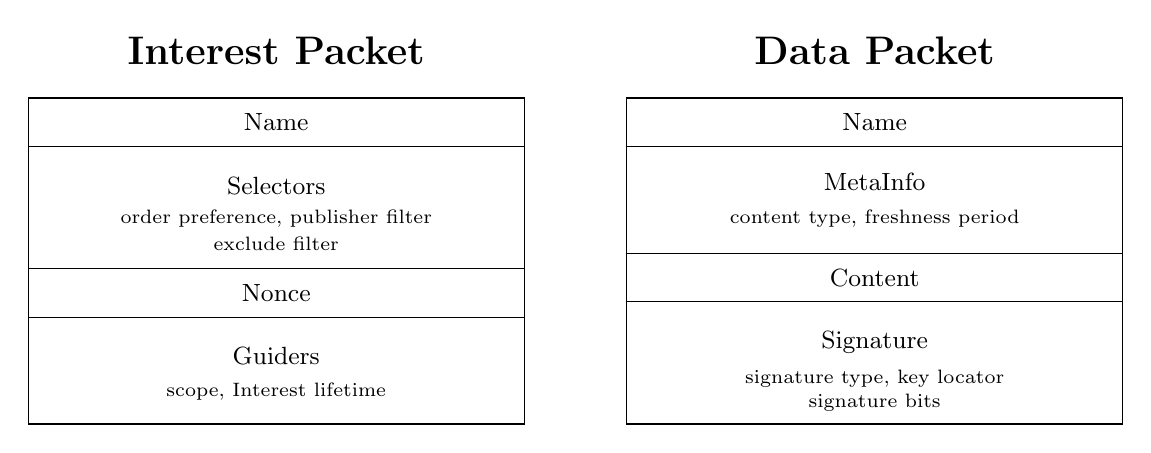
\begin{tikzpicture}[font=\small, every node/.style={align=center}]
\def\w{6.3}
\def\xA{-6.6}
\def\xB{1.0}
\node[font=\Large\bfseries] at (-3.45,2.95) {Interest Packet};
\draw (\xA,2.35) rectangle ++(\w,-0.62);
\node at (-3.45,2.04) {Name};
\draw (\xA,1.73) rectangle ++(\w,-1.55);
\node at (-3.45,1.24) {Selectors};
\node[font=\scriptsize] at (-3.45,0.82) {order preference, publisher filter};
\node[font=\scriptsize] at (-3.45,0.50) {exclude filter};
\draw (\xA,0.18) rectangle ++(\w,-0.62);
\node at (-3.45,-0.13) {Nonce};
\draw (\xA,-0.44) rectangle ++(\w,-1.35);
\node at (-3.45,-0.92) {Guiders};
\node[font=\scriptsize] at (-3.45,-1.38) {scope, Interest lifetime};

\node[font=\Large\bfseries] at (4.15,2.95) {Data Packet};
\draw (\xB,2.35) rectangle ++(\w,-0.62);
\node at (4.15,2.04) {Name};
\draw (\xB,1.73) rectangle ++(\w,-1.35);
\node at (4.15,1.28) {MetaInfo};
\node[font=\scriptsize] at (4.15,0.82) {content type, freshness period};
\draw (\xB,0.38) rectangle ++(\w,-0.62);
\node at (4.15,0.07) {Content};
\draw (\xB,-0.24) rectangle ++(\w,-1.55);
\node at (4.15,-0.76) {Signature};
\node[font=\scriptsize] at (4.15,-1.22) {signature type, key locator};
\node[font=\scriptsize] at (4.15,-1.52) {signature bits};
\end{tikzpicture}%
}
\caption{NDN Interest 和 Data packet 结构的简化图，根据 NDN 架构论文~\cite{ndn}重新绘制。}
\label{fig:ndn-packets-ch}
\end{figure}

数据驱动获取和网内缓存很有用，但服务调用不只是获取单个对象。多个
provider 需要发现某个 request 已经发布，user 需要先收集 ACK metadata 再
选择 provider，长时间运行的任务还需要状态诊断。因此，NDNSF 使用 NDN
Sync，尤其是 NDN-SVS 实现的 State Vector Sync，让 user 和 provider 发现
新发布的服务消息，而不需要把服务绑定到固定端点
~\cite{li2018brief,moll2022sok,ndnsvs-github}。在 NDNSF 中，Sync 不是服
务语义本身，而是 Request、ACK、Selection 和 Response 等命名 Data 消息的
发布和发现底座。

实现层面，NDNSF 构建在标准 NDN 软件栈上。NFD 提供本地 forwarder 和 Face
抽象，\texttt{ndn-cxx} 提供 C++ 应用开发所需的名字、packet、Face、签名、
验证和 segmented object retrieval~\cite{ndn-cxx}。这些库使 NDNSF 可以使
用普通 NDN 名字和 packet，而不需要重新发明一套传输格式；同时也支持应用
通过 reference 传递大 artifact：模型、视频录制、图片、日志和中间推理数
据可以被分段成命名 Data packet，被签名、可选加密、按名字获取，并在小型
service-request payload 之外独立验证。

访问控制方面，NDNSF 使用 NAC-ABE，将 NDN 命名和属性基加密结合起来，使
服务级授权可以围绕名字表达，而不是围绕传输连接表达~\cite{dulal2023nacabe}。
NDNSF 将这一能力与 controller 分发的权限、服务级属性和每次调用的一次性
token 结合起来。由此，NDN 提供数据中心通信底座，而 NDNSF 提供服务层
runtime：谁可以调用服务、谁可以提供服务、如何选择 provider、如何保护消
息，以及如何把大型命名对象附加到服务 workflow 中。

\begin{table}[H]
\centering
\caption{NDN 基础组件如何对应 NDNSF 机制。}
\label{tab:ndn-to-ndnsf-ch}
\begin{tabularx}{\textwidth}{p{0.30\textwidth}X}
\toprule
NDN 基础组件 & NDNSF 机制 \\
\midrule
Data packet & Request、ACK、Selection 和 Response 是承载在命名 Data 中
的服务消息对象。 \\
Interest & Interest 用于按名字获取 Data；NDN-SVS 使用 Sync Interest 宣告
数据集更新。 \\
Data 签名和基于名字的 trust & service message、permission 和大对象可以独
立于返回路径或缓存位置被验证。 \\
FIB/PIT/CS 转发与缓存 & 服务相关数据可以按名字获取，并在移动、缓存和间
歇连接场景下保持语义。 \\
NDN Sync / SVS & user 和 provider 可以发现新发布的服务事件，而不需要把
服务绑定到固定 endpoint。 \\
分段 Data 获取 & 大模型、视频、日志和中间 tensor 通过 reference 携带，而
不是塞进小型 service payload。 \\
NAC-ABE 和命名属性 & 服务级权限和保密策略围绕名字与属性表达，而不是围
绕传输信道表达。 \\
\bottomrule
\end{tabularx}
\end{table}

\section{研究缺口}

因此，本文关注的研究缺口存在于 NDN 通信 primitives 和面向服务应用语义之
间。NDN 提供命名 Data、签名、缓存、转发状态、分段获取和基于 Sync 的发
现；但它本身并不定义 user 如何调用命名服务、授权 provider 如何发布
readiness、ACK metadata 如何收集、一个或多个 provider 如何被选择、replay
如何防止，以及大对象如何附着到服务 workflow。NDNSF 将这些功能上升为可复
用 framework mechanisms，而不是让每个应用各自拼接 glue code。

\section{论文论点}

本论文认为，动态面向服务应用和主机中心服务框架之间存在反复出现的不匹配：
应用希望围绕命名服务、命名能力、命名数据和可验证结果组织逻辑，而底层网
络栈通常暴露的是地址、信道和端点。数据中心服务框架可以通过在 NDN 名字
和可验证 Data packet 之上显式提供服务调用、授权、服务提供者选择、协作和
大对象获取抽象，缓解这种不匹配。

NDNSF v0.1 是本博士论文已经完成的核心贡献之一，并证明这一方向具有可行
性。后续博士论文工作将在这一基础上，将 NDNSF 扩展成面向真实动态服务应
用的框架，并通过两个高压力应用领域验证其设计：

\begin{itemize}
  \item \textbf{UAV 网络应用}代表移动、命令敏感、实时的 service-container
  workload。这类应用同时涉及间歇连接、命令授权、遥测、实时视频、录制、
  目标检测和多无人机任务协作。
  \item \textbf{分布式 AI 推理应用}代表 artifact 密集、多阶段的计算/数据
  协作 workload。这类应用需要在多个服务提供者之间协调模型分片、运行时
  artifact、中间张量、大数据对象和协作计划。
\end{itemize}

论文的核心命题是：如果服务、数据、权限和协作计划都可以被命名和验证，
那么应用就可以在动态环境中更自然地发现服务、选择提供者、保护数据并从故
障中恢复。

\section{研究问题}

\begin{enumerate}[label=RQ\arabic*., leftmargin=*]
  \item 主机中心服务框架在移动性、服务发现、安全验证和数据获取方面会产
  生哪些结构性问题？其中哪些可以通过数据中心服务命名和可验证 Data 得到
  缓解？
  \item NDNSF 应如何把服务调用、授权、服务提供者选择、协作和大对象获取
  抽象成通用 framework 机制，而不是让每个应用重新设计一个专用 NDN 协议？
  \item 当 NDN 服务请求可以发布给多个服务提供者，并通过 ACK metadata、
  provider selection 和 provider collaboration 解析时，会产生哪些可靠性、安
  全性和延迟 tradeoff？Targeted invocation 和 compensation 等支撑机制应如
  何使用？
  \item UAV 网络应用如何在移动、命令敏感、实时 service-container 场景下
  评估 NDNSF？
  \item 分布式 AI 推理如何在 artifact 密集、多阶段、计算/数据协作场景下
  评估 NDNSF？
\end{enumerate}

\subsection{预期回答形式}

本文预期以如下形式回答这些问题。RQ1 应识别一组反复出现的服务应用问题：
这些问题不只是已有系统的工程实现缺口，而是服务被绑定到 host、session 或
channel 后产生的结构性后果。RQ2 应说明 NDNSF 可以把服务调用、授权、
provider selection 和 provider collaboration 暴露为可复用框架机制；本地组
合和大数据引用则作为支撑性抽象，避免每个应用重新设计专用 NDN 协议。RQ3 应刻画 one-to-many request
publication、ACK metadata、provider selection 和 provider collaboration 在
什么情况下能改善可靠性，以及 Targeted invocation 或 compensation 等支撑
机制何时用于控制延迟和恢复成本，同时不削弱安全检查。RQ4 应说明 UAV
workload 如何在移动性、命令敏感性、实时视频和多无人机协作压力下检验同
一组框架机制。RQ5 应说明分布式推理如何在 artifact provisioning、tensor
dependency exchange、provider role assignment 和长时间分布式执行压力下
检验同一组机制。

\section{预期贡献}

本文预期贡献如下：

\begin{enumerate}[leftmargin=*]
  \item 一个面向 NDN 的通用、安全、动态服务框架 NDNSF。
  \item 以服务提供者协作为核心的 NDNSF 扩展，并包含 Targeted invocation、
  trusted local service composition 和大数据引用等支撑机制。
  \item 一个基于 NDNSF 的 UAV service-container 应用，覆盖飞控、遥测、
  视频、加密录制、目标检测和协作巡逻服务。
  \item 一个基于 NDNSF 的分布式 AI 推理应用，覆盖模型切分、服务计划、
  基于 reference 的 artifact exchange 和自动协作计划生成。
  \item 使用 MiniNDN、SITL UAV 实验和部分真机验证对 NDNSF 及应用原型进
  行评估。
\end{enumerate}

\section{Proposal 范围边界}

为保持 proposal 的边界清晰，本文将 NDNSF v0.1 视为博士论文已经完成的核
心基础成果，而不是最终完整系统。NDNSF v0.1 已经建立了 data-centric
service framework 的基本架构，并证明了这一方向的可行性。后续博士论文工
作将在这一基础上，把 NDNSF 扩展成经过应用验证的 framework。主要框架扩
展是 provider collaboration：多个已授权 provider 如何发现 request、发布能
力或状态、被选择、交换状态或 artifact，并共同完成一个服务任务。Targeted
invocation、trusted local invocation 和 large-data reference 是让这一协作服务
模型在低延迟调用、同进程组合和大对象 workload 中可落地的支撑机制。这些
机制不是 UAV 专用或 AI 专用功能，而是拟作为 NDNSF 通用机制完成并评估的
设计。

因此，本论文的核心问题不是能否实现两个应用，而是 NDNSF 是否能够提供可
复用的数据中心服务机制，并且这些机制能否在两个差异很大的 workload 中保
持成立。

UAV 应用用于验证 NDNSF 是否适合作为移动、命令敏感、实时系统的
service-container framework。它的设计会检验结构化遥测、任务、视频和安
全信息、Targeted 飞控命令、自适应直播视频、加密本地录制、目标检测服务
组合和多无人机协作巡逻。DistributedInference 应用用于验证 NDNSF 是
否适合作为 artifact 密集、多阶段计算/数据协作的 framework。它的设计会检
验自动模型计划生成、基于 reference 的模型和 activation artifact、可预测可预取
对象名称，以及基于 tensor DAG 的依赖驱动执行。也就是说，UAV 和
DistributedInference 不是两个孤立 demo，而是用于验证同一个 data-centric
service framework thesis 的两个互补压力场景。

这两个应用也会反向提出 NDNSF 的框架需求。UAV workload 会压力测试低延
迟命令调用、结构化命令状态、service-container 组合和视频大数据引用；
DistributedInference workload 会压力测试依赖驱动协作、artifact reference、
provider role assignment 和长任务 selection 诊断。因此，应用工作在论文中
有双重意义：它们本身是有价值的应用系统，同时也是验证和完善 provider
collaboration 这一核心 NDNSF 扩展的主要方法。

\chapter{面向服务应用的框架}
\label{chap:soa-ch}

\section{本章目的}

本章不是要对所有服务框架做宽泛综述，而是回顾已有系统已经解决了什么，并
说明为什么在这些系统存在的情况下仍然需要 NDNSF。关键问题不是 gRPC、ROS、
微服务或 NDN Service Call 是否有用；它们显然有用。关键问题是：为什么动
态、安全、协作型应用仍然需要另一个框架。

\section{主机中心 RPC 和微服务框架}

RPC 系统（如 gRPC~\cite{grpc}）、HTTP/REST 系统~\cite{fielding2000rest}
以及微服务平台已经成为构建分布式软件的主流方式。它们提供类型化 API、传
输绑定、负载均衡、服务注册和生产环境工具。当服务能够由稳定端点标识、信
道能够建立并保持、安全性能够表示为信道安全加服务端授权时，这些系统工作
得很好。

然而，在移动和间歇连接环境下，这种抽象不再自然。UAV 视频服务用户关心
的是来自无人机 A 的最新帧，而不是无人机 A 当前通过哪个 IP 地址可达。分
布式推理客户端关心的是某个模型阶段的服务名，而不是固定 GPU 服务器。任
务规划应用可能需要任意满足角色要求的无人机，而不是某个预配置端点。主机
中心框架可以支持这些场景，但发现、重试、状态跟踪和应用特定协调的负担会
转移到框架之外。

\subsection{这些系统已经解决的问题}

RPC 和微服务系统解决了 NDNSF 不应忽视的若干问题。首先，它们提供熟悉的
编程模型：服务有接口、请求类型、响应类型、错误处理和 deadline。其次，
围绕 gRPC 和 REST 的生产系统提供成熟的负载均衡、日志、监控、部署和版本
管理工具。第三，TLS 等信道安全机制提供了保护客户端服务器通信的实用方式。
对于稳定云服务，这些能力通常已经足够。

NDNSF 并不试图否定这些工程经验，而是关注当服务提供者移动、间歇连接、复
制或嵌入资源受限边缘环境时，哪些假设会失效。在这些场景中，一次服务调用
不仅是信道操作，也是关于哪个提供者当前被授权、可达、有能力且值得选择的
决策。现有框架可以实现这些逻辑，但通常需要分散在服务发现系统、负载均衡
器、应用重试、中间件插件和服务特定策略代码中。

\subsection{NDNSF 需要解决的开放问题}

第一个问题是端点依赖。即使现代 service mesh 用逻辑服务名隐藏 IP 地址，
底层通信仍然依赖主机中心路由到达某个端点。第二个问题是数据生命周期。一
旦响应、视频 chunk、模型分片或遥测日志被存储到原信道之外，应用必须额外
定义验证和加密模型。第三个问题是服务提供者多样性。RPC 通常在请求发送前
就选择单个服务器；NDNSF 则允许多个提供者观察请求、决定是否 ACK，并暴露
帮助用户选择的元数据。这些差异促使我们设计数据中心服务框架，而不仅仅是
另一个 IP endpoint wrapper。

\section{机器人中间件和服务组合}

ROS 和 ROS2~\cite{ros,ros2} 等机器人中间件为机器人组件提供了更贴近应
用的模型。节点可以发布 topic、调用 service，并通过标准消息类型交互。与
早期 ROS 相比，ROS2 改进了 QoS 控制和部署灵活性。这些框架对 UAV 应用
非常重要，因为它们将传感器、控制、遥测和感知视为可组合模块。

剩余缺口是：机器人中间件不是通用的数据中心网络安全框架。Trust anchor、
证书部署、数据静态保护、多提供者选择和跨域服务授权并不是其核心抽象。此
外，部署在地面站、多架无人机和间歇无线链路上的 UAV 应用仍然需要在单一
本地机器人域之外可靠工作的命名、验证和恢复机制。

\subsection{对 UAV 服务容器的启示}

ROS 对本论文特别重要，因为它表明机器人应用天然是面向服务的。UAV 系统
不是单一通信流，而是由飞控命令、遥测流、摄像头帧、地图、任务规划、目标
检测、日志和健康监测共同组成。ROS 式组合验证了 UAV 软件应该被分解成服
务的思想。

然而，NDNSF 面向的是不同层次。ROS 和 ROS2 是本地及分布式机器人组件的
强中间件，而 NDNSF 关注基于 NDN 的命名、安全、网络可见服务调用。在拟
实现的 UAV 应用中，无人机 app 仍可被视为服务容器，但地面站命令、遥测发
现、视频获取和跨无人机协作等外部交互使用 NDNSF 服务名和数据中心验证。
因此，NDNSF 不是飞控或机器人中间件的替代品，而是连接这些组件并使它们能
在动态 NDN 环境中运行的网络服务框架。

\section{消息队列和事件系统}

消息队列和发布订阅系统在时间上解耦生产者和消费者~\cite{messagequeue}。
它们适合遥测、日志、异步工作流和弹性后端处理。这与 NDNSF 相关，因为许
多服务应用同时包含请求响应动作和事件流。例如，无人机可能以服务请求形式
接收命令，同时异步发布遥测或视频元数据；分布式推理流水线也可能在处理用
户请求的同时发布中间结果和执行事件。

然而，许多消息队列部署依赖 broker 或逻辑中心化基础设施。安全性通常通过
broker 访问控制和信道加密执行，而不是由可在任何存储或转发位置验证的数
据对象来保证。对于移动或断连边缘环境，broker 的可用性和部署位置可能成为
限制。此外，队列本身并不定义用户如何在多个服务提供者中选择、如何验证提
供者是否被授权提供特定服务，或如何以可验证数据形式获取大型服务 artifact。

\section{NDN 计算和服务框架}

NDN 已经为面向服务系统提供了有用原语：层次化名字、数据驱动获取、网内
缓存、自适应转发和 Data 签名~\cite{ndn}。NDN 上的服务框架必须弥合这些
原语和应用层服务语义之间的差距。已有 NDN 工作探索了该设计空间的多个区
域。

\subsection{函数中心计算}

Named Function Networking（NFN）将计算视为一等命名对象，并将函数表达式
嵌入名字~\cite{nfn}。这种模型很强大，因为它允许计算和数据获取在命名系
统内组合，也展示了内容名和计算名深度集成的可能性。

代价是复杂性。函数中心命名具有很强表达能力，但执行语义、信任、缓存和部
署也更难推理。UAV 控制、实时视频和分布式 AI 推理需要显式服务授权、服务
提供者选择、长时间状态和应用定义的执行策略。因此，NDNSF 选择服务调用抽
象，而不是完全通用的函数表达式抽象。

\subsection{Serverless 和边缘型 NDN 框架}

NFaaS 将 NDN 推向 serverless computing，把函数视为可在边缘位置执行的可
部署单元~\cite{nfaas}。其他边缘框架，例如面向信息中心 IoV 的 CFEC，也探
索低延迟微服务执行和动态放置~\cite{cfec}。这些系统突出一个重要方向：服
务执行应靠近用户、数据源或资源丰富的边缘节点。

开放问题在于，动态放置只是服务应用支持的一部分。应用还需要稳定 API、用
户和提供者授权、多提供者选择、大对象处理以及清晰部署流程。NDNSF 关注这
些运行时服务语义。它也可以与未来放置机制共存；例如，放置算法可以决定哪
些无人机、存储组件或推理提供者应发布某个 NDNSF 服务。

\subsection{远程调用框架}

RICE 在 ICN 中提供远程方法调用，使用 handshake 和 thunk 表示计算参数与
结果~\cite{rice}。NSC 为 NDN 提出 Named Service Calls，并提供类似 RPC
的远程执行抽象~\cite{nsc}。这些系统与 NDNSF 目标接近，因为它们直接处理
服务调用，而不只是内容获取。

主要限制是它们没有提供本论文目标应用所需的完整机制。NSC 主要是一对一：
调用者联系 executor，协议不是围绕同时服务提供者发现、ACK 元数据和多提供
者选择设计的。RICE 提供更强调用语义，但需要修改 forwarding plane。NDNSF
将框架保留在应用/运行时层，并使用 NDN Data 发布和 Sync 支持一对多服务请
求传播，而不修改 NFD。

\subsection{应用特定 NDN 框架}

其他 NDN 系统聚焦特定领域。DNMP 使用 NDN 同步和层次 topic 构建安全网络
测量框架~\cite{dnmp}。MIA-NDN 探索 NDN 中以微服务为中心的 Interest 聚合
~\cite{miandn}。SECaaS 研究 multi-access edge 中的 security-as-a-service
~\cite{secaas}。这些项目表明，当名字和应用语义一起设计时，NDN 能够适配
实际服务型 workload。

限制在于通用性。应用特定框架常常假设特定数据类型、服务领域、聚合模式或
部署拓扑。NDNSF 则试图提供可复用框架层，支持 UAV 控制、视频、目标检测、
分布式推理、存储和协作等不同服务。拟实现的 UAV 和 DistributedInference
应用将检验该框架是否足够通用，而不仅仅适用于一个精心调优的应用。

\subsection{安全和访问控制机制}

NDN 默认对 Data packet 签名，但签名本身不能回答所有服务问题。服务框架
必须决定谁可以请求服务、谁可以提供服务、哪些数据应加密、密钥如何分发以
及重放消息如何被拒绝。属性基加密和 NAC-ABE 展示了细粒度访问控制如何与
NDN 数据名集成~\cite{goyal2006abe,dulal2023nacabe}。这些思想是 NDNSF 的核心。

开放问题是与服务工作流的集成。如果访问控制被临时添加到每个应用中，每个
应用都必须分别处理权限获取、加密属性、消息验证和防重放。NDNSF 将这些机
制纳入运行时：ServiceController 分发权限，服务消息根据服务级属性保护，
一次性 user/provider token 将 ACK、selection、Targeted fast path 和
response 绑定到当前调用。

\section{NDN 服务系统}

NDN Service Call（NSC）~\cite{nsc} 和其他 NDN 应用框架表明，NDN 能够在
没有 IP 端点绑定的情况下支持服务调用。NDN 的 Interest/Data 交换、基于名
字的路由、网内缓存和数据签名解决了 IP 系统中的若干问题。因此，这些系统
证明 NDN 是服务的有前景基础。

剩余缺口是：现有 NDN 服务系统尚未提供一个通用运行时来同时结合：

\begin{itemize}
  \item 通用动态服务 API；
  \item controller 授权的用户和提供者权限；
  \item 一对多请求发布；
  \item 服务提供者 ACK 元数据；
  \item 应用定义的选择策略；
  \item 自适应 admission control；
  \item 大数据引用；
  \item 服务提供者协作；
  \item 可在真实场景中评估的 service container。
\end{itemize}

\section{设计模式和权衡}

相关工作显示出几个反复出现的设计模式。首先，服务框架必须将服务名与提供
者位置解耦。第二，大型输入和输出应表示为命名数据对象，而不是直接嵌入小
请求 payload。第三，服务状态通常不能只依赖 NDN Pending Interest Table，
因为服务执行可能长时间、多步骤或协作式。第四，安全性必须成为调用工作流
的一部分，而不是事后附加。

这些模式也暴露出权衡。函数中心名字表达力强，但部署困难；serverless 放置
灵活，但需要编排；RPC 式调用易于理解，但倾向一对一执行；broker 系统在时
间上解耦，但可能引入基础设施依赖。NDNSF 的设计点是将类似 RPC 的开发者
API 与 NDN 的数据中心名字、签名 Data、基于 Sync 的发布和应用可见的提供
者选择结合起来。

\section{开放问题}

表~\ref{tab:framework-gaps-ch} 总结了推动 NDNSF 的开放问题。

\begin{table}[H]
\centering
\caption{现有面向服务框架中的开放问题。}
\label{tab:framework-gaps-ch}
\begin{tabularx}{\textwidth}{p{0.25\textwidth}X}
\toprule
问题 & 重要性 \\
\midrule
端点绑定 & 移动服务和间歇连接提供者应按名字和能力调用，而不是依赖稳定主机地址。 \\
一对多调用 & 可靠性和协作常常需要多个提供者听到请求，并允许用户选择一个或多个提供者。 \\
数据中心安全 & 数据在静态存储时也应保持签名、可验证和可选加密，而不只是经过安全信道时受保护。 \\
提供者授权 & 用户不仅要验证自己是否能调用服务，也要验证被选择的提供者是否有权提供服务。 \\
提供者选择 & 负载、队列长度、位置和可用性等元数据应成为服务流程的一部分。 \\
大数据 & 模型、视频、图片、日志和中间张量不应被迫塞进小请求 payload。 \\
协作 & 任务可能需要多个提供者、补偿请求或部分结果聚合。 \\
操作验证 & 真实系统需要可重复的证书、路由、配置和实验环境，以便在 toy
example 之外验证框架。 \\
\bottomrule
\end{tabularx}
\end{table}

NDNSF 旨在使用 NDN 名字、可验证 Data、基于 Sync 的发布和服务级授权来解
决这些问题。

本章通过把 related work 转化为 framework requirements 来支持 RQ1，而不
只是列出已有系统。它也为 RQ2 和 RQ3 铺垫：哪些性质必须由 NDNSF runtime
提供，而不能让每个 UAV 或推理应用分别重新实现。

\chapter{NDNSF 框架}
\label{chap:ndnsf-ch}

\section{设计目标}

NDNSF 的设计目标如下：

\begin{enumerate}[leftmargin=*]
  \item \textbf{通用服务抽象。}应用应能用统一 service name、请求对象和
  响应对象表达服务，而不是依赖为每个服务生成的静态 stub。
  \item \textbf{数据中心安全。}服务消息和权限对象应作为 NDN Data 被签名、
  加密和验证。
  \item \textbf{协作与韧性。}框架应支持多个提供者、选择性 ACK、自定义选
  择和补偿请求。
  \item \textbf{低延迟路径。}对已知提供者的控制命令，应通过 Targeted
  invocation 减少消息轮次，同时保持权限和 token 验证。
  \item \textbf{操作验证。}框架应支持 MiniNDN 评估、选择性真机实验、证
  书 bootstrap 和可复现配置。
\end{enumerate}

\section{NDNSF v0.1 基线}

NDNSF v0.1 包括：

\begin{itemize}
  \item ServiceController、ServiceUser 和 ServiceProvider 运行时；
  \item 通用动态 C++ 服务 API；
  \item 基于 NDN Data 和 Sync 的 Request、ACK、Selection 和 Response
  消息；
  \item 基于 NAC-ABE 的服务级访问控制；
  \item 提供者权限和用户权限获取；
  \item 选择性 ACK 和自定义选择策略；
  \item 自适应 admission control；
  \item 与 NSC 和 gRPC 的 MiniNDN 对比评估。
\end{itemize}

这个 baseline 的意义在于，它已经把数据中心服务框架必须协调的主要部分连
接起来：service naming、service-message publication、用户和提供者授权、
加密服务 payload、provider metadata、provider selection 和 response
verification。换言之，NDNSF v0.1 不只是一个 API 草图，而是一个可运行的
runtime，展示了如何把 NDN name、Sync、signed Data、NAC-ABE attribute 和
service-level policy 组合成一个完整服务调用 workflow。因此，本 proposal
可以把重点放在扩展和验证 framework，而不是从零开始设计。

图~\ref{fig:ndnsf-v01-architecture-ch} 总结了 v0.1 baseline 中的三个运
行时角色。Controller 管理 policy 并分发权限；Provider 订阅有权限处理的
请求并发布服务结果；User 发布请求、收集 ACK metadata、选择 provider 并
验证 response。这个角色划分是后续 UAV service container 和分布式推理服
务协作的基础。

\begin{figure}[H]
\centering
\begin{subfigure}[t]{0.78\textwidth}
  \centering
  \includegraphics[width=\linewidth]{../named-data-network-service-framework-paper/figures/NDNSF_ServiceController.png}
  \caption{Controller}
\end{subfigure}

\vspace{0.8em}

\begin{subfigure}[t]{0.78\textwidth}
  \centering
  \includegraphics[width=\linewidth]{../named-data-network-service-framework-paper/figures/NDNSF_ServiceProvider.png}
  \caption{Provider}
\end{subfigure}

\vspace{0.8em}

\begin{subfigure}[t]{0.78\textwidth}
  \centering
  \includegraphics[width=\linewidth]{../named-data-network-service-framework-paper/figures/NDNSF_ServiceUser.png}
  \caption{User}
\end{subfigure}
\caption{作为 proposal baseline 的 NDNSF v0.1 运行时角色。}
\label{fig:ndnsf-v01-architecture-ch}
\end{figure}

\section{作为核心扩展的服务提供者协作}

NDNSF v0.1 之后最核心的扩展是 provider collaboration。在协作服务中，一个
逻辑 request 不一定只由单个 endpoint 完成，而可以由多个已授权 provider
共同参与。Provider 可以发布 ACK metadata，例如可用性、队列状态、位置或
role capability；User 可以在 ACK collection interval 之后选择一个或多个
provider；当一个逻辑任务只完成了一部分时，应用可以发出 compensation
request。对于耗时较长的 selection，User 还应能诊断被选中的 provider 当
前是未收到 selection、排队中、执行中、出错，还是已经发布 response。

这个协作模型应保持 application-independent。多无人机巡逻可以用它分配任
务段并从部分失败中恢复；分布式推理可以用它分配模型 role 并协调中间
artifact。两类应用都不应把自己的领域语义写入 NDNSF core。NDNSF 提供的
通用语义是 request publication、provider metadata、provider selection、
authorization、status diagnosis 和 response verification；具体领域工作由
应用定义。

\section{通用动态 API}

NDNSF 当前使用通用动态 API。服务提供者注册 typed handler：

\begin{lstlisting}[language=C++]
provider.addHandler<RequestT, ResponseT>(
    ndn::Name("/ObjectDetection/YOLOv8"),
    handler);
\end{lstlisting}

服务用户请求服务：

\begin{lstlisting}[language=C++]
user.RequestService<RequestT, ResponseT>(
    providers,
    ndn::Name("/ObjectDetection/YOLOv8"),
    request,
    onResponse,
    onTimeout,
    timeoutMs,
    strategy);
\end{lstlisting}

这个 API 将应用对象与框架消息分离。应用数据位于 typed request/response
对象或 RequestMessage/ResponseMessage payload 中。框架负责命名、发布、
加密、验证、provider selection 和 timeout。

\section{服务消息模型}

NDNSF v0.1 使用四类框架消息，将服务发布、provider admission、provider
selection 和结果返回分开。这一消息模型是 one-to-many service design 的
核心：同一个请求可以被多个有权限的 provider 观察到，provider 可以在真正
执行之前暴露可用性和运行时 metadata，用户则显式选择一个或多个 provider。

\begin{table}[H]
\centering
\caption{NDNSF v0.1 服务消息。}
\label{tab:ndnsf-message-model-ch}
\begin{tabularx}{\textwidth}{p{0.30\textwidth}p{0.16\textwidth}X}
\toprule
消息 & 生产者 & 作用 \\
\midrule
RequestMessage & User & 发布命名服务请求和应用 payload。 \\
RequestAckMessage & Provider & 表示 provider 是否愿意处理请求，并携带用于
选择的运行时 metadata。 \\
SelectionMessage & User & 选择一个或多个 provider，并用 provider token
将请求绑定到被选中的 provider。 \\
ResponseMessage & Provider & 被选中的 provider 返回服务执行结果。 \\
\bottomrule
\end{tabularx}
\end{table}

\begin{table}[H]
\centering
\caption{四类消息携带的代表性字段。}
\label{tab:ndnsf-message-fields-ch}
\begin{tabularx}{\textwidth}{p{0.30\textwidth}X}
\toprule
消息 & 代表性字段 \\
\midrule
RequestMessage & service name、request ID、requester identity、payload、
UserToken \\
RequestAckMessage & service name、request ID、provider identity、status、
message、metadata payload、回显的 UserToken、ProviderToken \\
SelectionMessage & service name、request ID、selected provider identity、
ProviderToken \\
ResponseMessage & service name、request ID、provider identity、result
payload、回显的 UserToken \\
\bottomrule
\end{tabularx}
\end{table}

这些字段保持 service-independent。应用相关数据留在 payload 或 typed
request/response 对象中；框架则使用 service name、request ID、identity
和一次性 token 完成授权检查、防重放和 response verification。

\section{服务调用流程}

普通 NDNSF 服务调用包括以下步骤：

\begin{enumerate}[leftmargin=*]
  \item 用户发布 RequestMessage，并携带一次性 UserToken。
  \item 有权限的提供者解密请求，检查 provider permission，并根据 ACK 策
  略决定是否回应。
  \item 提供者发布 RequestAckMessage，返回 UserToken、一次性
  ProviderToken 和 ACK metadata。
  \item 用户在 ACK timeout 内收集候选者，根据策略选择一个或多个提供者。
  \item 用户发布 SelectionMessage，并携带被选中提供者的 ProviderToken。
  \item 提供者验证 ProviderToken，执行服务并发布 ResponseMessage。
  \item 用户验证 response 中的 UserToken 并交付应用结果。
\end{enumerate}

该流程支持一对多发现、应用自定义选择和防重放保护。对已知提供者的低延迟
调用，Targeted API 先通过 normal bootstrap 获取一批 token pair，然后后续
请求可走 REQUEST 到 RESPONSE 的 fast path。

\section{安全模型}

NDNSF 使用 controller 授权的权限模型。ServiceController 维护用户和提供者
policy，向目标 identity 生成加密的 PermissionResponse。服务消息根据服务
级授权 namespace 映射到 NAC-ABE attribute。一次性 user/provider token 将
调用流程绑定到特定 request，防止 replay。

图~\ref{fig:ndnsf-policy-example-ch} 展示了 NDNSF 中 provider policy 和
user policy 的关系：provider permission 决定一个实体可以提供哪些命名服
务，user permission 决定一个实体可以访问哪些命名服务。本文后续 UAV 和
DistributedInference 扩展都沿用这种以 service name 为中心的 policy 模型，
同时补充更明确的 trust root、publisher namespace 和部署流程。

\begin{figure}[H]
\centering
\includegraphics[width=0.82\textwidth]{../named-data-network-service-framework-paper/figures/policy-examples.png}
\caption{NDNSF provider 和 user access-control policy 示例。}
\label{fig:ndnsf-policy-example-ch}
\end{figure}

该模型区分：

\begin{itemize}
  \item \textbf{用户授权}：用户是否可以请求某服务；
  \item \textbf{提供者授权}：提供者是否可以提供某服务；
  \item \textbf{消息机密性}：只有具有相应 attribute 的实体可以解密服务
  消息；
  \item \textbf{消息完整性和来源认证}：NDN Data signature 和 trust schema
  保护消息；
  \item \textbf{防重放}：UserToken 和 ProviderToken 一次性使用。
\end{itemize}

\subsection{采用 ABE-backed 服务授权的理由}
\label{sec:abe-rationale-ch}

NDNSF 采用 ABE-backed 授权，是为了支持面向授权服务提供者的保密发现，
并将服务权限管理与身份签名凭证分离。这是针对 NDNSF 调用流程的设计取舍，
并非 ABE 全面优于角色授权的结论。执行授权决定实体是否可以调用或提供某项
服务；内容机密性决定谁能读取受保护的消息内容。签名验证、服务权限检查和
调用状态检查仍是不同的要求。

\paragraph{发现阶段的保密性。}
在选择 Provider 之前，User 发布 discovery descriptor（发现描述），其中
包含 Provider 决定是否返回 positive ACK 所需的位置、截止时间和资源要求。
例如，附近 UAV 需要知道观察区域和到达时限才能决定是否参与，但此时不需要
完整应用输入。ABE 无需逐一列出 Provider 身份，即可将发现描述的读取权限
限制为获准提供该服务的 Providers。这里的保密对象是缺少相应解密能力的外部
观察者；获准但最终未被选中的 Providers 仍可读取。内容加密不隐藏外层 Data
名称或流量模式。在请求级机密性路径中，完整应用输入及其解密材料通过
Selection 限定给选中的
Providers。Trust Schema 本身不加密内容；角色授权方案也可以配合 ABE 或
服务组加密来实现发现阶段的保密性。

\paragraph{权限聚合与凭证复用。}
KP-ABE 将属性关联到密文，将访问策略编码到解密密钥
（DKEY）中~\cite{dulal2023nacabe}。NDNSF 使用
\texttt{/SERVICE/<service>} 表示 Provider 的服务解密权限，使用
\texttt{/PERMISSION/<service>} 表示 User 的调用相关解密权限。在同一授权
机构和 ABE 参数代际内，一个实体的多项服务权限被合并为 OR 策略，编码到
单独为该实体签发的 DKEY 中，同时复用其身份签名凭证。DNMP 则通过角色签名
密钥和 Trust Schema 约束命令的目标与动作~\cite{dnmp}。已有角色可以覆盖多项
权限；不同权限需求可能要求调整角色分配、凭证或规则，但不意味着每项服务
都必须建立新角色。

作为对照，我们提出的每服务角色证书方案会为实体获准承担的每项服务角色签发
证书。User 使用相应服务角色密钥签名 Request 和 Selection Data，Provider
使用相应密钥签名 ACK 和 Response Data。验证方检查服务、消息类型、证书
所授角色、证书状态及调用状态，内容保密则由配套加密机制提供。ABE 避免了
这些额外的服务专用签名凭证，但 DKEY 仍需签发和更新，其大小及处理成本可能
随策略复杂度增长。证书方案也能复用凭证，因此凭证对象数量较少本身不足以
证明总成本更低。

\paragraph{为何继续使用 ABE-backed challenges？}
Requester Challenge（实现中的 \texttt{UserToken}）和 Provider Challenge
（\texttt{ProviderToken}）用于检查参与者在当前交换中是否具有相应的服务和
调用权限解密能力。签名标识参与身份，匹配检查和一次性状态检查拒绝不匹配或
重放的消息。这沿用了属性化权限管理，而不必另外增加服务角色签名凭证，但
并非没有额外成本：保密发现已需要 Provider DKEY，而 User 的调用权限 DKEY
和 challenge 处理仍是额外授权成本。ABE 保密配合角色证书授权同样是有效的
替代方案。

\subsection{运行时权限撤销}
\label{sec:authorization-withdrawal-ch}

当前运行时通过 Controller 签名的授权状态以及调用处理点上的检查实现权限
撤销。参与者需要获取并验证更新后的状态，才能执行新公布的权限撤销。
ABE 参数轮换和 DKEY 更新保护随后使用新代际加密的交换。目前轮换作用于整个
Controller 的 ABE 参数代际，其他仍获授权的成员也可能需要刷新 DKEY；
这不是无需更新其他成员的撤销方案。

DNMP 描述了通过轮换加密密钥限制后续测量数据访问，但没有详细给出可对应
比较的在线命令授权撤销协议~\cite{dnmp}。角色证书对照方案可以撤销相关凭证，
并要求执行节点检查签名的撤销状态或拒绝过期证书。这是在验证方取消凭证
所代表的权限，而不是物理取回已分发的证书。两类方案都需要传播更新信息，
也都无法收回已披露的密钥或明文。

定向集成测试已检验 NDNSF 的运行时撤销检查，包括身份级、证书级和服务级
撤销。这些测试支持已覆盖运行时边界上的行为，不代表整个网络中的瞬时撤销，
也不能证明其成本低于证书方案。后续评估应测量状态传播延迟、拒绝生效延迟、
重新分发密钥的流量，以及对未撤销成员的影响。因此，运行时状态验证和密钥
轮换使 NDNSF 支持权限撤销，同时带来明确的状态传播和重新分发密钥的成本。


\section{已完成基础：NDNSF v0.1 评估}

已完成的 NDNSF 评估在 MiniNDN 中将 NDNSF 与 NSC 和 gRPC 进行对比。评估
关注有线、丢包、间歇提供者、无线移动、自适应 admission、选择性 ACK 和
自定义选择场景中的服务延迟和成功率。证据支持的结论是有条件的：在丢包、
间歇 provider 和单一 endpoint 绑定容易失效的场景中，provider 多样性可以
提高可靠性；这并不等价于 NDNSF 在所有动态环境中都具有更高的终端成功率或
更低的延迟。

最有说服力的证据来自 endpoint binding 或单一 provider 变脆弱的场景。在
1\% link loss 的有线网络中，NDNSF 和 gRPC 保持 100\% success rate，而
NSC 因缺少有效 loss recovery 出现超过 12\% 的 request failure。在有线多
provider 的间歇失效实验中，provider failure probability 为 20\% 时，
NDNSF 仍保持 99.46\% success rate；失效概率为 30\% 时仍有 96.70\%，而单
provider baseline 会下降到约三分之二或更低。无线移动表中的数值属于已投稿
NDNSF v0.1 的历史诊断，拓扑、provider 数量和计时来源与当前公平的 Spec171
四-provider campaign 不完全一致，因此不能把它们作为当前 mobility superiority
的直接证据。当前校正后的单 AP、50\,m 覆盖、2\,m/s 移动、三 seed 复现实验中，
NDNSF success rate 为 75.33\%，相对 gRPC 的 71.78\% 提高 3.55 个百分点，
相对 NSC 的 70.11\% 提高 5.22 个百分点；但在 50\,m/15\,m/s 和
100\,m/15\,m/s 条件下并不占优，因此这里应表述为条件性结果，而非普遍
mobility 优势。Adaptive
admission 和 Selective ACK 进一步说明 runtime metadata 的价值：过载时
admission control 将 P95 latency 保持在 270\,ms 以下；当最近 provider 过
载时，Selective ACK 将 success rate 从 1.82\% 提高到 100\%。这些结果共同
支撑较窄的结论：one-to-many invocation、provider metadata 和显式 selection
能在保持数据中心安全的同时，为特定 provider-diversity 和间歇可用性场景提供
可靠性收益；当前证据还不足以支持普遍的无线 mobility 优势。

\begin{table}[H]
\centering
\caption{从已投稿 NDNSF v0.1 历史评估中总结的代表性可靠性结果；无线行不作为当前公平 mobility superiority 的证据。}
\label{tab:ndnsf-v01-reliability-ch}
\begin{tabularx}{\textwidth}{p{0.27\textwidth}p{0.21\textwidth}ccc}
\toprule
场景 & 条件 & NSC & gRPC & NDNSF \\
\midrule
有线多 provider 间歇失效 & 10\% 失效概率 & 83.25\% & 83.35\% & \textbf{99.82\%} \\
有线多 provider 间歇失效 & 20\% 失效概率 & 66.58\% & 66.69\% & \textbf{99.46\%} \\
有线多 provider 间歇失效 & 30\% 失效概率 & 49.92\% & 65.36\% & \textbf{96.70\%} \\
无线移动 provider & 100\,m AP range & 45.42\% & 45.23\% & \textbf{96.25\%} \\
无线移动 provider & 150\,m AP range & 68.75\% & 68.05\% & \textbf{100.00\%} \\
无线移动 provider & 200\,m AP range & 88.33\% & 87.14\% & \textbf{100.00\%} \\
\bottomrule
\end{tabularx}
\end{table}

\begin{table}[H]
\centering
\caption{从已投稿 NDNSF v0.1 评估中总结的代表性机制结果。}
\label{tab:ndnsf-v01-mechanisms-ch}
\begin{tabularx}{\textwidth}{p{0.24\textwidth}p{0.29\textwidth}X}
\toprule
机制 & Baseline 行为 & NDNSF 行为 \\
\midrule
100 RPS offered load 下的 adaptive admission & 关闭 admission control 时，P95 latency 达到 4254.39\,ms，timeout rate 达到 3.55\%。 & 开启 admission control 后，实际 admitted rate 限制在约 81 RPS，P95 latency 为 268.12\,ms，timeout rate 为 0.00\%。 \\
最近 provider 过载时的 Selective ACK & ACK-all 机制把 2250 个请求中的 2209 个选到最近但过载的 provider，success rate 只有 1.82\%。 & Selective ACK 抑制过载 provider 的 ACK，把 selection 转移到可用 provider，并达到 100.00\% success rate。 \\
真机间歇可用性实验 & 单 provider NSC/gRPC 在绑定 provider 半程不可用时 success rate 接近 50\%。 & NDNSF 在两个 provider 中动态选择，10 RPS 下达到 74.62\%，30 RPS 下达到 73.73\%，接近预期可用窗口。 \\
\bottomrule
\end{tabularx}
\end{table}

\section{NDNSF v0.1 的局限}

NDNSF v0.1 证明了方向可行，但还没有完全覆盖受控框架测试之外的动态服务
应用需求。
推动后续博士论文工作的主要局限包括：

\begin{itemize}
  \item \textbf{已知提供者的低延迟控制}：normal
  Request/ACK/Selection/Response workflow 适合 provider discovery，但发
  往已知无人机或设备的控制命令需要更快的 Targeted path，同时仍要保留授
  权和防重放保护。
  \item \textbf{服务提供者协作}：v0.1 支持 provider selection，但更大的
  任务需要多个 provider 协作、处理部分失败并发出 compensation request。
  \item \textbf{Service-container 组合}：真实应用通常在同一受信任进程内
  包含多个服务。这些服务需要高效本地组合，但不能向远程 caller 暴露绕过
  网络安全机制的路径。
  \item \textbf{大 artifact}：v0.1 service payload 不适合承载模型、录制
  视频、图片或中间张量。应用应在 service payload 中放置 typed object
  reference，再使用 NDN 原生 segmented retrieval 获取大型签名和加密对象。
  \item \textbf{操作验证}：v0.1 展示了安全模型，但更广泛的验证还需要更
  清晰的证书 bootstrap、trust-schema 指导、配置流程和可复现实验。
  \item \textbf{应用级验证}：v0.1 的 MiniNDN 评估证明核心框架可运行，但
  博士论文还需要评估该设计是否能支撑 UAV 和分布式推理这类高压力 workflow。
\end{itemize}

\section{Provider Collaboration 的支撑机制}

以下机制用于支撑 provider collaboration 在特定运行条件下成立。它们由 UAV
和分布式推理 workload 驱动，但不是独立博士论文主线，也不应成为应用专用
shortcut，而应保持为通用 framework mechanism。

\subsection{Targeted Invocation}

对于面向已知 provider 的控制服务，例如 MAVLink 命令，完整 ACK/Selection
流程会增加延迟。Targeted invocation 使用 normal 流程进行首次 bootstrap，
获取一批一次性 token pair，随后每个 request 携带未使用的 ProviderToken，
response 返回对应 UserToken。这样可以减少消息轮次，同时保留权限验证和防
重放语义。

\subsection{Trusted Local Invocation}

Service container 内部的服务组合不需要走网络。同一受信任进程内的一个服
务组件调用另一个内部服务组件时，不应发布 NDNSF Request。拟实现的本地调
用机制支持同进程 trusted local invocation，包括同步和异步调用。该路径不
生成 wire message，不使用 NAC-ABE，也不消耗 token；外部节点不能要求
provider 使用该路径，它只用于同一受信任进程内的服务组合。

\subsection{大数据引用抽象}

服务请求 payload 不应承载模型、视频、图片或大张量。拟采用的通用模式是：
数据生产者先把对象分段发布为具名 NDN Data，然后在 NDNSF request 或
response 中只放 typed object reference。该 reference 可以包含对象名字、
对象类型、version 或 session id、digest、expected size、final segment 信
息、source type 以及可选加密 metadata。接收方收到 request/response 后，
使用 NDN 原生 segmented fetching，例如 ndn-cxx SegmentFetcher 逻辑，按名
字拉取对象。

该抽象应作为 NDNSF 的通用机制，而不是某个特定存储服务的 API。小型
request/response payload 仍适合控制消息和紧凑 typed object；当 payload
变成模型、视频、activation 或日志这类大 artifact 时，同一个逻辑服务调用
应携带 reference，而不是直接携带字节。应用或 helper 可以把 payload 转换
成命名 Data segment，对这些 segment 签名并可选加密，然后通过 NDNSF 传递
typed reference。这样，服务选择、授权、token 检查和 timeout 诊断仍属于
普通 NDNSF 路径，而大字节传输则走 NDN 原生 named-data retrieval 路径。

同一种 reference 格式应能覆盖 UAV 录制、相机 artifact、模型分片、runtime
artifact、中间 activation 和日志。因此，UAV-APP 与 DistributedInference
可以共享同一套框架级大数据词汇：object type、object name、producer、
session 或 version、size、digest、final segment hint 和可选 encryption
metadata。这避免在 service payload 中嵌入应用特定的裸 Data-name 字符串，
也让不熟悉 NDN packet 细节的应用能够审查大对象行为。

该设计可以选择使用持久化存储，但存储在本 proposal 中只是大对象实现支撑
组件，而不是单独的研究主线。如果使用持久化存储，它应保存 opaque 的 NDN
Data segment；这些 Data 已由应用或框架 helper 命名、签名，并可选加密。
安全性不由存储专用接口单独承担，而是由 NDNSF 通用混合加密、签名、token、
权限和 trust-schema 验证保护 service message 及其引用的数据。Discovery
metadata 仍可作为应用层发现和验证加速工具存在，但大对象传输本身应基于
typed object reference 和 NDN 原生分段获取。

本章通过预览可复用 NDNSF 机制来支持 RQ2，包括安全服务调用、provider 授
权、provider collaboration 以及相关支撑机制。它也支持 RQ3，因为 provider
collaboration 会引入可靠性、安全性和延迟 tradeoff，而支撑机制需要在不削
弱核心服务语义的前提下控制开销。

\chapter{基于 NDNSF 的 UAV 网络应用}
\label{chap:uav-ch}

\section{为什么 UAV 网络需要服务框架}

UAV 应用是 NDNSF 的重要验证 workload，因为它同时包含移动性、实时控制、
视频、分布式感知、多机协作和安全约束。一个 UAV 网络可能包括地面站、多
架无人机、摄像头、flight controller、目标检测服务、录制能力和任务规划组
件；这些组件暴露的能力天然适合用 service 表达。

在本博士论文中，UAV workload 更具体地用于压力测试移动和命令敏感场景下
的 provider collaboration。地面站可能需要发现多架无人机，为同一个 mission
选择一个或多个 provider，向已知无人机发出 targeted command，在某个任务
段失败后发出 compensation request，并在不把大对象塞进 RPC payload 的情况
下获取视频或录制对象。因此，UAV-APP 的作用不是单纯展示 UAV 功能，而是
验证 NDNSF framework：provider collaboration、授权、selection status、低
延迟支撑机制和大数据引用能否在面向操作者的 service container 中协同工作。

在 IP 上开发 UAV 网络应用面临一组重复问题：

\begin{itemize}
  \item \textbf{地址绑定。}无人机 identity 和 IP 地址可能随移动、链路切
  换或 NAT 改变。
  \item \textbf{服务发现。}地面站需要知道哪些无人机提供飞控、遥测、视频
  或录制服务。
  \item \textbf{命令授权。}飞控命令必须仅允许授权用户调用并防止重放。
  \item \textbf{数据验证。}遥测、视频和任务结果应可独立验证。
  \item \textbf{断连恢复。}无人机可能间歇性离线，任务应能重新分配。
  \item \textbf{协作复杂度。}多无人机巡逻要求任务拆分、分配、补偿和结果
  汇总。
\end{itemize}

\section{UAV 服务}

拟实现的 NDNSF-UAV-APP 将 UAV 网络建模为 service-container application。
地面站和无人机 app 可以共享协议和工具代码，但各自运行不同服务。部署相
关的 identity、service name、运行角色、摄像头行为和飞控 backend 应通过
应用配置表达，而不是固化在程序逻辑中。

\begin{table}[H]
\centering
\caption{拟实现 UAV 应用中的服务类型。}
\label{tab:uav-services-ch}
\begin{tabularx}{\textwidth}{p{0.27\textwidth}X}
\toprule
服务类型 & 目的 \\
\midrule
飞控服务 & arm、takeoff、land、goto、manual control 和通用 MAVLink execute。 \\
遥测和状态服务 & 报告 GPS、高度、电量、armed 状态、flight mode、readiness、摄像头可用性、链路状态和任务状态。 \\
视频控制服务 & 开启/关闭实时视频，协商 bitrate，并报告实际 streaming 参数。 \\
视频帧服务 & 发布编码帧或 chunk 作为 NDN Data，以支持低延迟播放。 \\
录制发现服务 & 授权发现无人机本地保存的加密视频对象。 \\
录制获取服务 & 通过 large-data reference 获取加密签名 NDN Data 对象。 \\
目标检测服务 & 从摄像头帧检测 car、truck 等目标，可在 GS 或 drone 上运行。 \\
协作巡逻服务 & 分配 waypoint、将任务划分给多架无人机、启动/停止任务并收集结果。 \\
\bottomrule
\end{tabularx}
\end{table}

\section{架构}

UAV 应用由两个主要角色组成：

\begin{itemize}
  \item \textbf{Ground station role}：提供操作者交互、基于地图的任务规
  划、遥测和视频观测、目标检测服务组合以及 NDNSF user 行为。
  \item \textbf{Drone role}：提供飞控适配、遥测发布、摄像头和视频发布、
  加密录制支持、任务执行以及 NDNSF provider 行为。
\end{itemize}

ServiceController 可运行在地面站或单独节点。真实部署中，证书和 trust
schema 应基于应用 namespace，例如 /muas/root 或 /example/uav，参与者证
书位于该 namespace 下。

地面站使用结构化运行时状态表示遥测新鲜度、任务进度、视频可用性和安全就
绪状态，使操作者可见状态和命令决策能够在多个独立命名服务之间保持一致。
已知无人机命令使用 Targeted invocation；协作巡逻、可选择 provider 的服
务和补偿请求使用 normal NDNSF selection。

\section{操作者工作流和状态纪律}

UAV 应用并不是为了替代已有地面站软件。它的目的，是验证 NDNSF 是否能够
支撑真实 UAV service workload。为了让这种验证有意义，GS 仍然必须回答实
际操作者关心的问题：当前选中哪架飞行器，它是否就绪和安全，当前命令或任
务处于什么阶段，遥测和视频是否新鲜，以及链路或设备失败后会发生什么。因
此，拟开展的 UAV 工作把 GS 设计为状态驱动的操作者控制台，而不是一组服
务调用入口。

\begin{table}[H]
\centering
\caption{NDNSF-UAV-APP 拟采用的操作者可见状态纪律。}
\label{tab:uav-operator-state-ch}
\begin{tabularx}{\textwidth}{p{0.23\textwidth}X}
\toprule
状态领域 & 拟实现行为 \\
\midrule
飞行器选择 & 在遥测、视频和服务更新异步到达时，GS 保持操作者选中的飞行器稳定。 \\
Readiness & GS 为 camera、flight controller、telemetry、mission、video、recording 和存储相关能力提供综合就绪视图。 \\
遥测新鲜度 & GS 区分当前、过期和缺失遥测，避免把旧数据误认为当前状态。 \\
命令生命周期 & 控制命令和任务命令应暴露可观察的进度、完成和超时结果，而不是只给出不透明的成功或失败消息。 \\
任务进度 & 巡逻任务应展示跨无人机的分配、进度、部分完成、取消和补偿行为。 \\
失败行为 & Timeout、设备失败和链路失败应暴露诊断信息，使操作者或应用策略能够决定下一步动作。 \\
\bottomrule
\end{tabularx}
\end{table}

\section{实时视频和录制}

地面站通过无人机的命名视频控制服务请求开启直播。无人机从摄像头读取视频
帧；实验环境也可以使用可重复的视频源模拟摄像头。视频应编码为
H.264/H.265 等可流式播放格式，再切成符合 NDN packet 限制的 chunk 发布。
每次直播应有 stream id 和单调递增 packet sequence；packet payload 中也携
带 stream metadata，使 GS 能拒绝旧 stream 或 cache 中的 stale packet。接
收端优先保持低延迟，并根据 RTT、bitrate、timeout pressure、decoder backlog
和 published/decoded gap 自适应调整预取窗口与跳帧策略。

录制和直播是不同功能。无人机可以在直播关闭时仍保持摄像头工作并本地录制。
录制对象表示为指向签名和加密 NDN Data segment 的 large-data reference。
GS 通过授权服务调用发现可用录制对象，再使用 segmented retrieval 按名字拉
取 segment，并在本地完成验证、解密和播放。这样持久化存储不需要理解服务
权限；service 授权和密钥信息由 NDNSF service message 处理，旧数据和重放
问题则通过 session id、stream id 和签名 Data 名字处理。

\section{飞控和安全}

飞控命令应通过 Targeted NDNSF API 发往指定无人机。无人机 app 将 MAVLink
message 转发给 PX4/SITL 或真实 flight controller~\cite{mavlink-survey,px4}。Manual control 是连续
控制消息，而不是普通长任务服务；它的 response 可以携带高度、GPS、速度、
电量和 flight controller state，让 GS 在手操时持续刷新状态。为了更接近
真机可用性，无人机应显示 readiness gate，包括 heartbeat、GPS/EKF、电量、
mode 和 arming check。安全策略包括：

\begin{itemize}
  \item manual control 超时后自动停止；
  \item 失联后进入 hold 或 land；
  \item emergency stop；
  \item 命令 ACK 解析，而不仅仅报告“已转发”；
  \item 真机实验必须遵守明确的物理安全约束。
\end{itemize}

\section{多无人机巡逻}

地面站允许用户在地图上放置 waypoint，然后将同一巡逻任务分配给多架无人机。
任务分配算法应按无人机数量和出发位置聚类 waypoint，使每架无人机负责一组
空间上接近的点。每架无人机完成任务后返回自己的起飞点并降落。如果某架无
人机 unavailable 或任务失败，地面站发出 compensation request，只补分配未
完成的子任务，而不是重新启动整个巡逻任务。

当前 UAV-APP 是研究原型，还不是已经可靠可用或经过安全认证的实战地面站
系统。这个边界对 proposal 很重要：后续实际使用、SITL 和选择性真机测试
仍可能暴露命令处理、遥测新鲜度、视频行为、安全策略、部署和操作者流程方
面的新需求或变化。这些发现本身也是研究价值的一部分，因为它们会反向推动
NDNSF framework 机制的完善和演化。

\section{评估计划}

UAV 应用评估将包括：

\begin{enumerate}[leftmargin=*]
  \item 单无人机 SITL：arm、takeoff、manual control、goto、land。
  \item 双无人机协作巡逻：waypoint 聚类、任务执行、返回起点。
  \item 直播视频：不同 bitrate、丢包、乱序和延迟下的播放质量。
  \item 本地录制和远程回放：录制发现授权、加密对象获取和播放。
  \item 失败恢复：断开一架无人机后补偿请求是否完成任务。
  \item 操作验证：PC + 多架无人机或 SITL 节点上的证书、路由和配置检查。
\end{enumerate}

本章通过把 UAV 定义为移动、命令敏感、实时 workload 来支持 RQ4，从而使
NDNSF 不只停留在 core framework regression。它也反向支持 RQ2 和 RQ3，
因为 UAV 行为会压力测试 Targeted invocation、provider collaboration、
timeout diagnosis 和 large-data reference。

\chapter{基于 NDNSF 的分布式 AI 推理}
\label{chap:inference-ch}

\section{研究动机}

分布式 AI 推理应用需要在多个节点之间协调模型 artifact、运行时依赖、中间
张量和最终结果。IP 环境下，开发者通常需要手动处理模型 shard 放置、artifact
下载、服务发现、任务调度、认证、数据传输和结果验证。随着边缘设备、无人
机、地面站和云节点共同参与推理，这些问题变得更加复杂。

在本博士论文中，分布式推理从另一个方向压力测试 provider collaboration。
这里的 provider 不是因为共享物理任务而协作，而是因为同一个推理任务可能
需要多个模型 chunk、runtime artifact、activation exchange 和按依赖排序的
执行步骤。因此，该 workload 检验的是 NDNSF 能否保持协作语义的通用性：
框架负责协调已授权 provider、大数据引用、状态诊断和结果验证；推理层负
责提供模型相关的 dependency graph 和 execution plan。

NDNSF 的服务命名和数据中心安全适合该问题。模型 shard、runtime artifact、
输入数据、中间张量和输出结果都可以被命名、签名、缓存和验证。服务调用可
以将推理任务分配给多个 provider，而大对象通过 typed reference 和 NDN
segmented retrieval 在 provider 之间传递；具体存储后端可以按部署需要选择。

\section{分布式 AI 推理方法}

已有分布式 AI 推理通常包括：

\begin{itemize}
  \item \textbf{数据并行}：多个节点运行相同模型，处理不同输入。
  \item \textbf{模型切分}：模型层或阶段被拆分到不同节点，类似 mobile、edge
  和 cloud 之间进行 DNN partitioning 的 split-computing 工作~\cite{neurosurgeon,ddnn}。
  \item \textbf{pipeline 推理}：多个阶段顺序处理，每个阶段由不同节点执行。
  \item \textbf{layer 或 operator partitioning}：根据计算、内存和中间
  activation 大小在更细粒度上切分模型图。
  \item \textbf{边云协作}：轻量前处理在边缘完成，重计算阶段在云或 GPU 节
  点完成。
  \item \textbf{early-exit 推理}：当中间结果已经足够可信时提前结束计算~\cite{branchynet}。
  \item \textbf{多模型协作}：检测、跟踪、分类或融合模型共同产生结果。
\end{itemize}

这些方法都需要命名 artifact、选择 provider、传输中间数据并验证结果。

\section{基于 NDNSF 的推理架构}

拟实现的 NDNSF-DistributedInference 将应用分层为：

\begin{itemize}
  \item APP 调用模型/推理 API；
  \item DistributedInference 层理解 model plan、role、stage、shard、runtime
  artifact、backend requirement 和依赖；
  \item large-data reference 层描述模型、runtime 和中间对象；
  \item NDNSF runtime 负责 Face、SVS、NAC-ABE、签名、权限、选择和 wire protocol。
\end{itemize}

在 ONNX 模型场景中，ONNX 提供机器学习模型的标准计算图表示~\cite{onnx}，
拟采用的路径如图~\ref{fig:di-plan-generation-ch} 所示。

\begin{figure}[H]
\centering
\begin{tikzpicture}[
  flowbox/.style={draw, rounded corners, align=center, minimum width=0.68\textwidth,
    minimum height=1.15cm, font=\footnotesize},
  flowarrow/.style={->, thick},
  arrowlabel/.style={font=\scriptsize, align=center}
]
  \node[flowbox] (onnx) at (0,0) {\textbf{ONNX graph}\\模型 operator、tensor 和图边};
  \node[flowbox] (dag) at (0,-1.90) {\textbf{Tensor dependency DAG}\\中间 tensor 的 producer-consumer 关系};
  \node[flowbox] (cuts) at (0,-3.80) {\textbf{Candidate split points}\\按 activation 大小和执行约束排序的切分边界};
  \node[flowbox] (chunks) at (0,-5.70) {\textbf{Chunk graph}\\可执行模型 chunk 和跨 chunk tensor 依赖};
  \node[flowbox] (plan) at (0,-7.60) {\textbf{NDNSF-DI collaboration plan}\\Provider role、artifact reference、对象名和 fallback policy};

  \draw[flowarrow] (onnx) -- (dag);
  \draw[flowarrow] (dag) -- (cuts);
  \draw[flowarrow] (cuts) -- (chunks);
  \draw[flowarrow] (chunks) -- (plan);
\end{tikzpicture}
\caption{从 ONNX 计算图自动生成 NDNSF-DistributedInference 协作计划的路径。}
\label{fig:di-plan-generation-ch}
\end{figure}

该路径根据真实模型图生成中间 tensor 依赖，而不是手写几条 pipeline edge。
同时，框架仍保留统一 splitter 输出接口，使 PyTorch、container、LLM 或非
ONNX 模型也能通过模型特定 splitter 接入。用户只需要调用推理服务；
provider 根据分配到的 role 通过 large-data reference 获取模型 chunk 和 runtime artifact，
预取可预测输入 tensor bundle，执行 chunk，然后发布输出 tensor bundle。

\section{自动协作计划生成}

拟完成的重要扩展是根据 AI 模型自动生成 collaboration plan。输入包括模型
图、tensor dependency DAG、candidate cut points、activation size、stage
latency、provider capability、可用 backend、网络状态和 artifact 位置。默认情
况下可以将 provider 视为同质化节点；未来可加入 CPU/GPU/内存/历史延迟等
profile。输出包括 role 分配、artifact 名字、中间对象名字、可预取对象名
和执行顺序。该计划不应由用户手写低层消息，而应由 DistributedInference 层
生成并交给 NDNSF 调用。

\section{依赖驱动执行器}

DistributedInference 的 provider 逻辑不应为 YOLO、全连接网络或某个 demo
单独手写通信流程。拟实现的 dependency-driven executor 读取当前 role 的
input edges，自动 fetch/merge 所需 tensor bundle，执行 ONNX 或模型特定
chunk，再按 output edges 发布 tensor bundle。该设计应支持 chain、fan-in
和 fan-out DAG。YOLO 2x2 和小型全连接网络因此是同一个依赖驱动执行器的验
证用例，而不是两套不相关的手写系统。

\section{当前原型状态}

当前原型已经实现并测试了一个基于 Ultralytics YOLOv8 software stack 的网
络级 YOLO 2x2 分布式推理路径~\cite{yolov8-ultralytics}。不同 provider
运行不同 ONNX chunk；模型和 runtime artifact 通过 large-data reference
进行 provisioning；provider 之间交换 activation reference，而不把大张量
塞进 service payload。回归验证会检查分布式输出是否与本地完整 pipeline
一致，并确认生成的 artifact metadata 可被应用审查。

该原型说明 NDNSF 机制已经可以支撑分布式推理，但它还不是最终的任意 ONNX
DAG 通用执行器。剩余研究工作是去掉 provider 逻辑中的模型特定假设，使用
ONNX tensor DAG 生成更真实的 fan-in/fan-out dependency graph，并让 planner
根据模型结构、artifact 放置和 provider/network profile 自动生成 service
policy。

\section{原型和评估计划}

原型将包括 YOLO split inference、小型全连接网络、2x2 provider 协作、
artifact reference 获取、结果一致性检查、fan-in/fan-out dependency execution
和 failure recovery。评估将测量：

\begin{itemize}
  \item 端到端推理延迟；
  \item 手写 policy 与自动生成 policy 的差异；
  \item chain execution 与 fan-in/fan-out dependency execution；
  \item artifact 获取时间；
  \item provider 利用率；
  \item 成功率；
  \item 与本地推理结果的一致性；
  \item artifact placement 对启动延迟的影响；
  \item provider failure 后的恢复时间。
\end{itemize}

本章通过把分布式推理定义为 artifact 密集、依赖驱动的 workload 来支持
RQ5，用于验证 NDNSF 是否能支撑多阶段计算/数据协作。它也反向支持 RQ2，
因为模型 artifact、provider role、自动计划和长任务 selection status 必须
保持通用，而不能退化成某个模型专用的通信协议。

\chapter{研究计划和时间线}
\label{chap:timeline-ch}

\section{已完成工作}

已完成工作包括 NDN 服务框架 survey、NDNSF v0.1、核心安全设计、提供者选
择、自适应 admission control 和初步 MiniNDN 评估。NDNSF v0.1 不是博士
论文之外的背景工作，而是本论文已经完成的第一阶段核心贡献。v0.1 之后的
UAV-APP、DistributedInference、provider collaboration 以及在真实 workload
中检验它所需的支撑机制，被视为在该核心贡献之上的应用驱动扩展和验证计
划，需要在博士论文中进一步完成和系统评估。
Repository 支持可以作为大对象实现组件使用，但不作为独立博士论文主线展开。

\section{剩余工作计划}

剩余博士论文工作现在主要是稳定、集成和评估，分为四条线：

\begin{enumerate}[leftmargin=*]
  \item \textbf{框架扩展}：以 provider collaboration 为核心收束 NDNSF 扩展，
  并稳定低延迟 Targeted invocation、trusted local composition、大数据引用和
  NAC-ABE 操作支持等支撑机制，重点是正确性、文档和 regression 覆盖。
  \item \textbf{UAV 应用}：稳定 GS 操作者工作流、service container 组织、
  MAVLink/PX4 集成、实时视频、加密录制、目标检测和多无人机巡逻，将其作
  为 NDNSF 的应用驱动验证。
  \item \textbf{DistributedInference}：完成 YOLO-style split inference 原型、
  自动 service plan、reference-based artifact exchange、provider assignment
  和 failure compensation，并冻结评估场景。
  \item \textbf{评估和写作}：运行最终 MiniNDN、SITL 和部分真机实验，同时
  把实验结果转化为博士论文章节。
\end{enumerate}

\section{评估矩阵}

最终评估需要把 framework thesis 与两个应用领域连接起来，并展示这些应用
如何验证和拓展 NDNSF 机制。表~\ref{tab:evaluation-matrix-ch} 总结拟收集
的证据。

\begin{table}[!htbp]
\centering
\caption{博士论文评估矩阵。}
\label{tab:evaluation-matrix-ch}
\begin{tabularx}{\textwidth}{p{0.09\textwidth}p{0.18\textwidth}p{0.31\textwidth}X}
\toprule
RQ & 评估领域 & 核心问题 & 证据 \\
\midrule
RQ1 & 框架缺口分析 & 哪些 host-centric service 问题是结构性的？哪些可以通过 data-centric naming 和可验证 Data 缓解？ & 对 RPC、机器人中间件、pub/sub、workflow 系统、NDN service approach、UAV 网络和分布式推理系统进行 related-work 对比，并归纳为 framework requirements。 \\
RQ2, RQ3 & NDNSF core & 数据中心服务调用是否在支持 provider collaboration 的同时保持授权、选择、防重放和 timeout 诊断语义？ & 权限、NAC-ABE routing、token replay、provider selection、collaboration status，以及 Targeted/local invocation 等支撑路径。 \\
RQ2 & 大数据引用 & 大对象能否通过 reference 传递而不改变安全语义？ & reference 格式验证、payload-to-Data 转换、segmented retrieval，以及 UAV 和分布式推理 artifact 的端到端兼容性检查。 \\
RQ4 & UAV 应用 & NDNSF 能否支持移动、命令敏感、实时 service-container workload？ & GS/Drone MiniNDN 测试、SITL MAVLink 检查、命令生命周期日志、视频稳定性、遥测新鲜度、录制获取、任务进度和失败恢复。 \\
RQ5 & 分布式推理 & NDNSF 能否支持 artifact 密集、多阶段的计算/数据协作？ & 本地与分布式输出一致性、ONNX graph summary、自动 policy 检查、reference-based artifact provisioning、activation exchange、fan-in/fan-out executor 测试和 provider failure 场景。 \\
RQ2, RQ4, RQ5 & 操作验证 & 框架能否在单一本地 build 之外被验证？ & 证书和路由流程、配置检查、可复现实验环境，以及选择性真机测试。 \\
\bottomrule
\end{tabularx}
\end{table}

\section{时间线}

\begin{table}[!htbp]
\centering
\caption{拟定博士论文时间线。}
\label{tab:timeline-ch}
\begin{tabularx}{\textwidth}{p{0.23\textwidth}X}
\toprule
阶段 & 工作内容 \\
\midrule
2026 年 8 月 31 日 & 稳定 NDNSF provider collaboration 及其 Targeted、local 和 large-data 支撑机制；冻结接口、可复现 build、回归覆盖与实验计划。 \\
2026 年 9 月 30 日 & 完成 UAV MiniNDN 与 SITL 评估，包括命令生命周期、遥测 readiness、实时视频、录制、任务工作流、compensation 与 recovery。 \\
2026 年 10 月 30 日 & 完成分布式推理评估，包括 ONNX policy、artifact 与 activation 交换、dependency-driven execution、输出一致性及 Provider-failure recovery。 \\
2026 年 11 月 13 日至 12 月 4 日 & 在论文写作并行推进的同时，于 11 月 13 日冻结已接受的数据集、配置、表格和图；于 12 月 4 日提交完整的导师审阅稿。 \\
2027 年 1 月 15 日至 2 月 5 日 & 于 1 月 15 日分发委员会审阅稿，解决导师意见，并于 2 月 5 日前完成毕业与 candidacy 手续；答辩公告须至少提前三周发布。 \\
2027 年 2 月中旬前 & 在委员会审阅和规定的公开通知期结束后举行博士论文答辩。 \\
2027 年 2 月 26 日 & 完成答辩后修改并取得委员会最终批准。 \\
2027 年 3 月 5--26 日 & 以 3 月 5 日为内部 ProQuest 提交目标，并在 3 月 26 日官方截止日前完成提交，以满足 Spring 2027 毕业要求。 \\
\bottomrule
\end{tabularx}
\end{table}

\section{风险和缓解}

\begin{itemize}
  \item \textbf{系统复杂度。}UAV 和 DistributedInference 都较复杂。缓解方式
  是保持 NDNSF core 泛化，将应用逻辑放在 service container 和应用层。
  \item \textbf{性能开销。}NAC-ABE、Sync 和日志可能影响延迟。缓解方式是
  在协作路径可能引入额外开销时使用 Targeted invocation、local invocation 和
  大数据引用等支撑机制，并结合采样日志和 benchmark profiling。
  \item \textbf{环境差异。}Ubuntu、NFD、ndn-cxx、NAC-ABE 和 PX4 版本可能
  影响复现。缓解方式是受控依赖环境、配置化流程和 CI/container 测试。
  \item \textbf{真机安全。}飞控实验风险高。缓解方式是先 SITL、再无桨测试、
  再小范围真机验证，并提供 emergency stop 和失联保护。
\end{itemize}

本章把研究问题与论文执行计划连接起来。它说明每个 RQ 都有对应的证据路
径，同时也保留 UAV 和 DistributedInference 在后续测试中发现新需求并反向
完善 NDNSF 设计的空间。

\chapter{结论}
\label{chap:conclusion-ch}

本 proposal 将 NDNSF 定位为面向动态、安全和协作网络应用的数据中心服务框
架。NDNSF v0.1 表明，NDN 可以支持带有授权、服务提供者选择和自适应行为
的通用服务抽象。拟开展的工作将下一步框架扩展集中在 provider
collaboration 上，并由 Targeted invocation、trusted local composition 和大数据
引用等机制支撑；该方向将通过 UAV 网络和分布式 AI 推理两个高要求应用领
域进行验证。

预期结果不仅是另一个应用实现，而是一套构建面向服务系统的框架和设计方法。
在该方法中，服务、数据、权限和协作计划都被命名并可验证，从而使应用能够
在动态环境中更可靠、更安全地运行。
UAV-APP 和 DistributedInference 的重要性在于它们从不同方向压力测试
NDNSF，并暴露框架必须提供的机制；但博士论文的核心贡献仍然是 NDNSF
framework、其机制设计，以及这些机制能够超越单一应用的证据。

\bibliographystyle{bibstyle}
\bibliography{ref}

\end{document}
